\section{Results}
\label{sec:results}

This section presents outcomes from the full experiment sweep, with explicit analysis and takeaway for each experiment.

\subsection{E1: Backhaul Savings}

\begin{figure}[H]
    \centering
    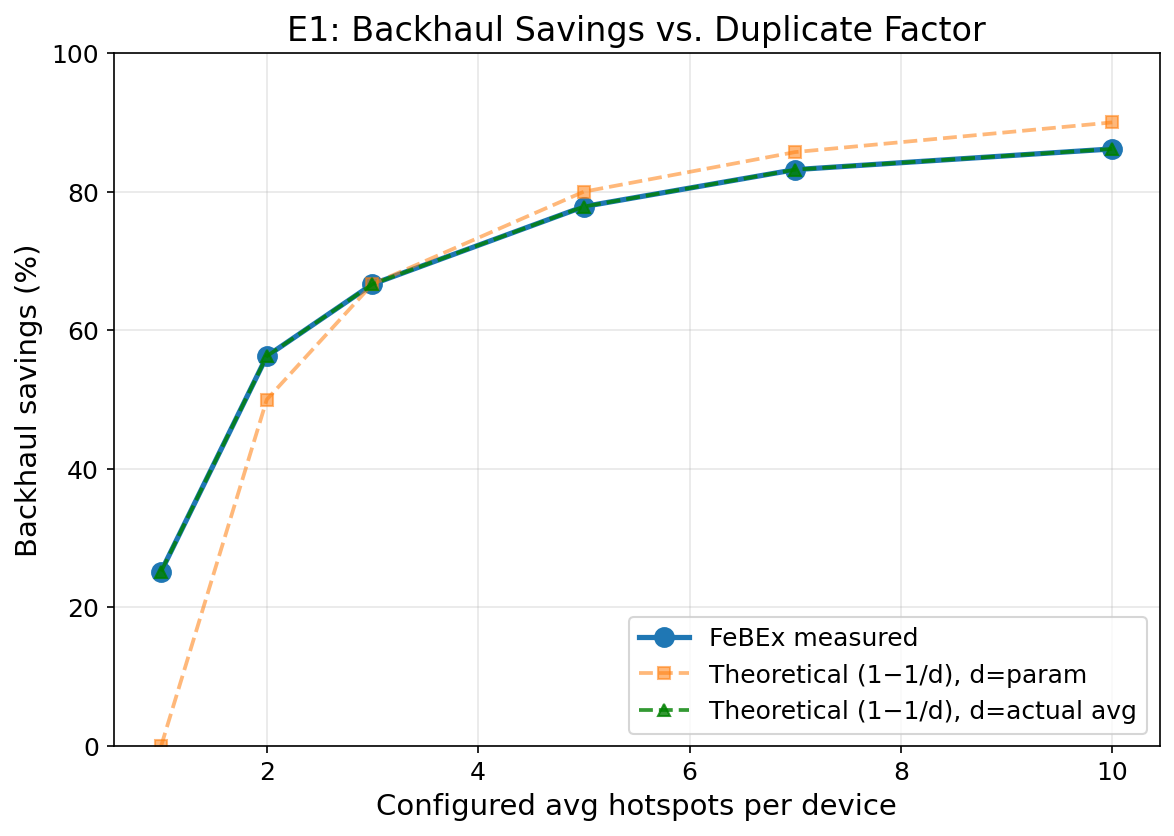
\includegraphics[width=0.85\linewidth]{figures/E1_backhaul_savings.png}
    \caption{Backhaul savings increases with duplicate factor and approaches theoretical limits.}
    \label{fig:e1-backhaul}
\end{figure}

FeBEx provides strong bandwidth reduction, with savings rising from low-duplication scenarios to high-duplication scenarios, matching the expected trend.

\textbf{Analysis:} Savings increase from approximately 25\% at low duplication to about 86\% at high duplication, closely tracking the expected theoretical limit as duplicate factor grows. Minor deviation at the highest stress point is consistent with BMv2 software effects under load.

\textbf{Takeaway:} In-network deduplication provides predictable and substantial backhaul reduction, with the largest gains in dense multi-gateway coverage regions.

\subsection{E2: Correctness (Delivery Ratio)}

\begin{figure}[H]
    \centering
    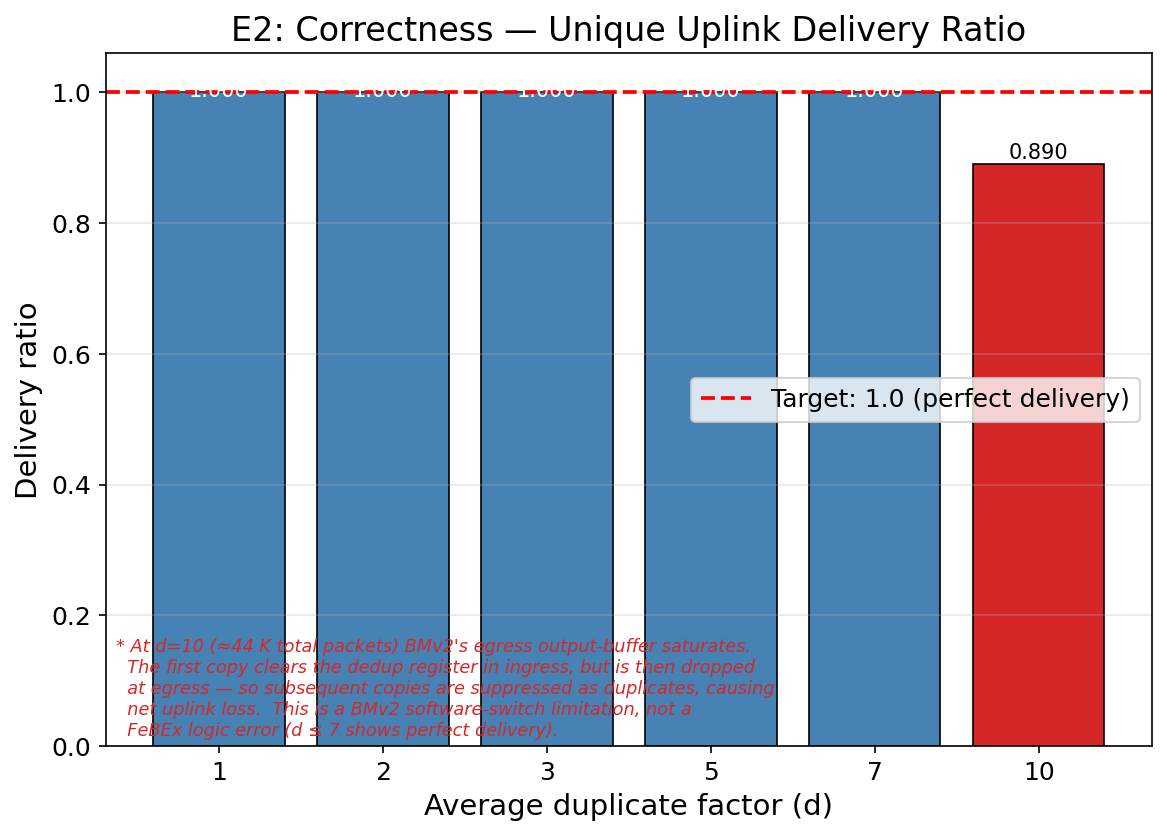
\includegraphics[width=0.78\linewidth]{figures/E2_correctness.png}
    \caption{Delivery ratio for unique uplinks under dedup ON.}
    \label{fig:e2-correctness}
\end{figure}

Delivery remains near-perfect for normal operating points; degradation only appears at extreme offered load where BMv2 software limitations dominate.

\textbf{Analysis:} Delivery ratio is effectively 1.0 for normal and moderate duplicate factors. The observed drop only at the highest stress point is aligned with BMv2 egress/buffer artifacts rather than a dedup logic error.

\textbf{Takeaway:} FeBEx correctness holds in realistic operating ranges; residual loss at extreme stress is a testbed bottleneck, not a design flaw.

\subsection{E3: Multi-Tenant Isolation}

\textbf{Analysis:} With 4 tenants and thousands of forwarded packets, no cross-tenant delivery violations were observed. DevAddr-prefix LPM steering remained consistent under dedup ON.

\textbf{Takeaway:} Tenant isolation is preserved end-to-end, so deduplication can be deployed without breaking multi-tenant routing boundaries.

\subsection{E4: City-Scale Scalability}

\begin{figure}[H]
    \centering
    
\includegraphics[width=0.9\linewidth]{figures/E4_scalability.png}
    \caption{Scalability across deployment sizes (devices/gateways).}
    \label{fig:e4-scalability}
\end{figure}

Across scales, FeBEx maintains substantial savings while throughput trends primarily reflect software-switch limits rather than algorithmic instability.

\textbf{Analysis:} Savings stay in the same band (roughly high-50s to high-60s percent) as topology size increases from small to large scenarios. Throughput peaks and then drops at the largest emulation size, indicating BMv2/Mininet saturation effects.

\textbf{Takeaway:} Dedup behavior scales stably with city-scale topology growth; observed throughput ceiling is primarily a software target limitation.

\subsection{E5: Register Sizing Sensitivity}

\begin{figure}[H]
    \centering
    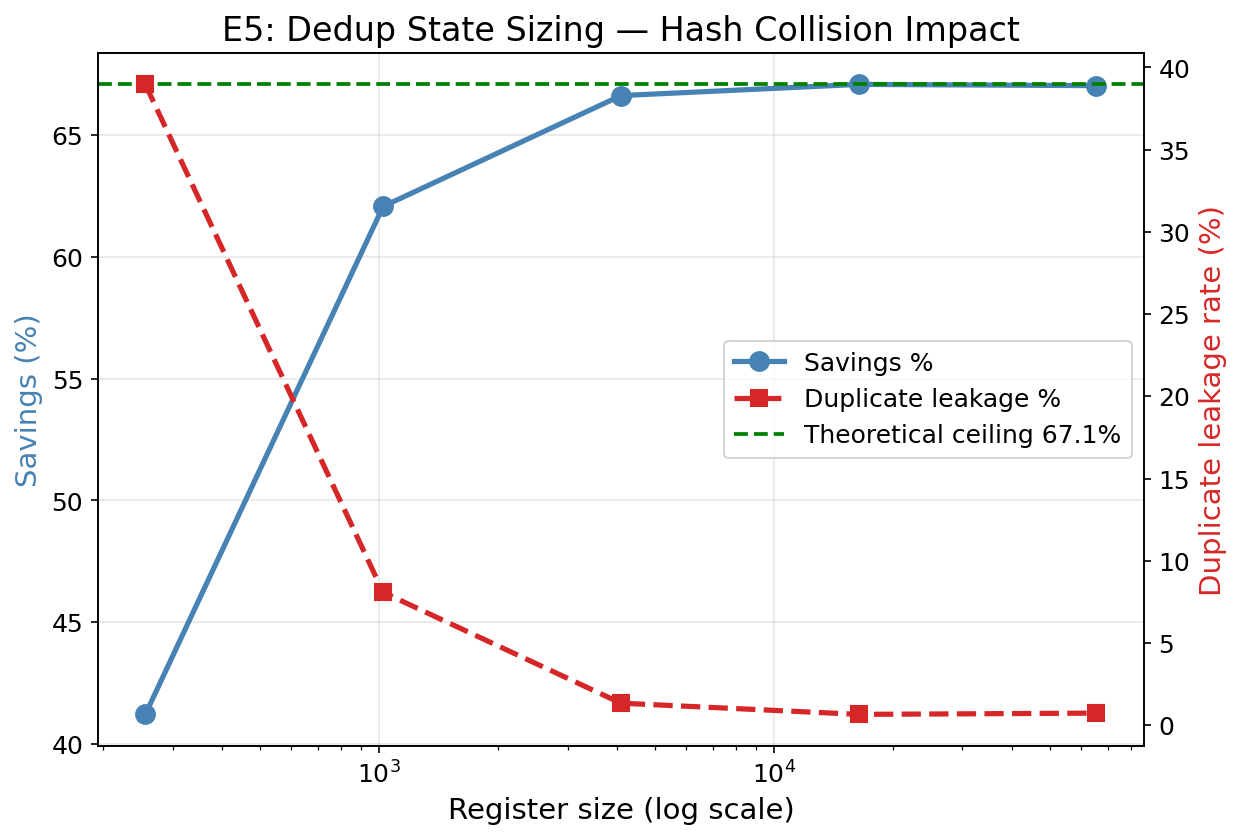
\includegraphics[width=0.9\linewidth]{figures/E5_state_sizing.png}
    \caption{Effect of register size on leakage and savings.}
    \label{fig:e5-sizing}
\end{figure}

Larger register arrays sharply reduce duplicate leakage. Results support a practical sizing rule of thumb: allocate at least $4\times$ the expected active device count.

\textbf{Analysis:} Leakage drops sharply when moving from very small tables to moderate ones (e.g., $256 \rightarrow 1024$), then plateaus beyond 4096 where additional memory yields diminishing return. Savings follow the same trend.

\textbf{Takeaway:} Right-sizing registers is the dominant control knob for collision-induced leakage; a practical deployment target is register size $\geq 4N$.

\subsection{E6: Epoch Interval Sensitivity}

\begin{figure}[H]
    \centering
    
\includegraphics[width=0.85\linewidth]{figures/E6_epoch_sensitivity.png}
    \caption{Impact of epoch interval on dedup effectiveness.}
    \label{fig:e6-epoch}
\end{figure}

Very short epochs increase boundary leakage; moderate intervals provide stable suppression with minimal stale-state effects.

\textbf{Analysis:} Leakage decreases monotonically as epoch interval increases, with near-zero leakage at 10s and above in our runs. Very short epochs (sub-second to 1s) amplify boundary effects.

\textbf{Takeaway:} Epoch interval should not be overly aggressive; 5--10 seconds provides a robust operating region for this workload class.

\subsection{E7: Payment Receipt Accuracy}

\textbf{Analysis:} Cloned cloud receipts maintain 1:1 correspondence with first-forwarded LNS packets, and gateway identifiers remain valid across the tested scenario.

\textbf{Takeaway:} FeBEx deduplication preserves attribution semantics required for Proof-of-Coverage/payment accounting.

\subsection{E8: Variant Comparison (V1/V2/V3)}

\begin{figure}[H]
    \centering
    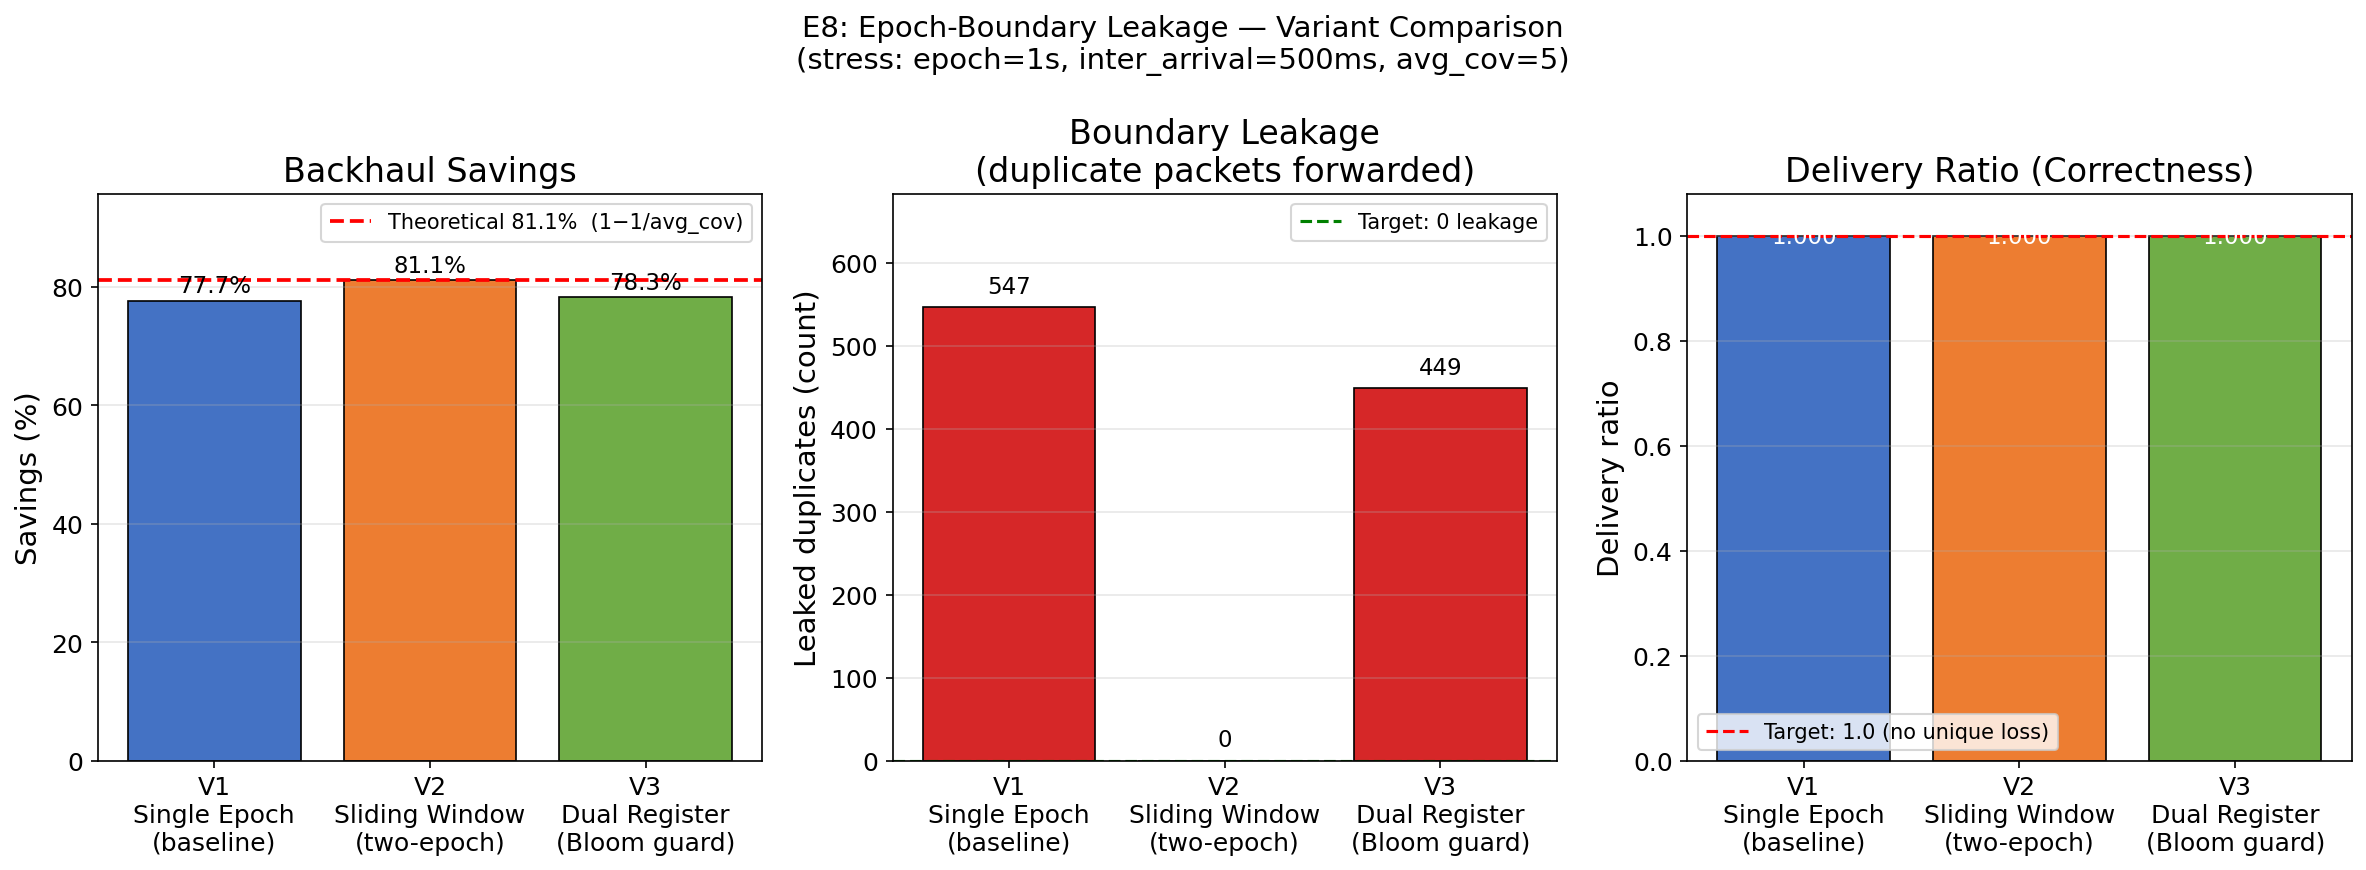
\includegraphics[width=0.85\linewidth]{figures/E8_variant_comparison.png}
    \caption{Variant comparison under boundary stress (V1 baseline, V2 sliding-window, V3 dual-register Bloom).}
    \label{fig:e8-variant}
\end{figure}

\textbf{Analysis:} Under boundary-stress settings, V2 (sliding-window) reaches the best behavior by suppressing cross-boundary duplicates. V3 improves collision-oriented behavior but does not remove boundary leakage by itself, so it remains below V2 on boundary-focused stress.

\textbf{Takeaway:} Use V2 when boundary leakage is the dominant issue; V3 is complementary for collision/false-positive robustness rather than a direct boundary fix.

\subsection{Summary}

Overall, the experiments show that FeBEx consistently reduces backhaul traffic, preserves correctness and tenant isolation, and offers clear operational tuning knobs (register size, epoch interval, and variant selection) for deployment.
